\documentclass[frenchb,DIV=14]{scrartcl}

\usepackage[utf8x]{inputenc}
\usepackage[T1]{fontenc}
\usepackage{lmodern}
\usepackage[binary-units=true]{siunitx}
% Color
% cfr http://en.wikibooks.org/wiki/LaTeX/Colors
\usepackage{color}
\usepackage[usenames,dvipsnames,svgnames,table]{xcolor}
\definecolor{dkgreen}{rgb}{0.25,0.7,0.35}
\definecolor{dkred}{rgb}{0.7,0,0}
\usepackage{graphicx}
\usepackage{url}
\usepackage{tikz}
\usepackage{pgfplots}
\usepackage{microtype}
\usepackage{xspace}

\usepackage{hyperref}
\usepackage{todonotes}
\usepackage{epstopdf}

\usepackage{multirow}
\usepackage{tabularx} % tabular with automatic line-break
\newcolumntype{Y}{>{\centering\arraybackslash}X} % centered column

\newcommand{\matlab}{\textsc{Matlab}}

% Math symbols
\usepackage{amsmath}
\usepackage{amssymb}
\usepackage{amsthm}
\DeclareMathOperator*{\argmin}{arg\,min}
\DeclareMathOperator*{\argmax}{arg\,max}

% Unit vectors
\usepackage{esint}
\usepackage{esvect}
\newcommand{\kmath}{k}
\newcommand{\xunit}{\hat{\imath}}
\newcommand{\yunit}{\hat{\jmath}}
\newcommand{\zunit}{\hat{\kmath}}
\newcommand{\uunit}{\hat{\umath}}

% Elec
\newcommand{\B}{\vec B}
\newcommand{\E}{\vec E}
\newcommand{\EMF}{\mathcal{E}}
\newcommand{\perm}{\varepsilon} % permittivity

\newcommand{\bigoh}{\mathcal{O}}
\newcommand\eqdef{\triangleq}

\DeclareMathOperator{\newdiff}{d} % use \dif instead
\newcommand{\dif}{\newdiff\!}
\newcommand{\fpart}[2]{\frac{\partial #1}{\partial #2}}
\newcommand{\ffpart}[2]{\frac{\partial^2 #1}{\partial #2^2}}
\newcommand{\fdpart}[3]{\frac{\partial^2 #1}{\partial #2\partial #3}}
\newcommand{\fdif}[2]{\frac{\dif #1}{\dif #2}}
\newcommand{\ffdif}[2]{\frac{\dif^2 #1}{\dif #2^2}}
\newcommand{\constant}{\ensuremath{\mathrm{cst}}}
\newcommand{\norm}[1]{\left\lVert#1\right\rVert}

\usepackage{babel}
% Listing
% always put it after babel
% http://tex.stackexchange.com/questions/100717/code-in-lstlisting-breaks-document-compile-error
\usepackage{listings}

% Put caption after babel
\usepackage{caption}
\usepackage{subcaption}

\definecolor{mygreen}{rgb}{0,0.6,0}
\definecolor{mygray}{rgb}{0.5,0.5,0.5}
\definecolor{mymauve}{rgb}{0.58,0,0.82}
\lstset{ %
  language=Matlab,
  backgroundcolor=\color{white},   % choose the background color; you must add \usepackage{color} or \usepackage{xcolor}
  basicstyle=\footnotesize,        % the size of the fonts that are used for the code
  breakatwhitespace=false,         % sets if automatic breaks should only happen at whitespace
  breaklines=true,                 % sets automatic line breaking
  captionpos=b,                    % sets the caption-position to bottom
  commentstyle=\color{mygreen},    % comment style
  deletekeywords={...},            % if you want to delete keywords from the given language
  escapeinside={\%*}{*)},          % if you want to add LaTeX within your code
  extendedchars=true,              % lets you use non-ASCII characters; for 8-bits encodings only, does not work with UTF-8
  frame=single,	                   % adds a frame around the code
  keepspaces=true,                 % keeps spaces in text, useful for keeping indentation of code (possibly needs columns=flexible)
  keywordstyle=\color{blue},       % keyword style
  otherkeywords={*,...},           % if you want to add more keywords to the set
  numbers=left,                    % where to put the line-numbers; possible values are (none, left, right)
  numbersep=5pt,                   % how far the line-numbers are from the code
  numberstyle=\tiny\color{mygray}, % the style that is used for the line-numbers
  rulecolor=\color{black},         % if not set, the frame-color may be changed on line-breaks within not-black text (e.g. comments (green here))
  showspaces=false,                % show spaces everywhere adding particular underscores; it overrides 'showstringspaces'
  showstringspaces=false,          % underline spaces within strings only
  showtabs=false,                  % show tabs within strings adding particular underscores
  stepnumber=1,                    % the step between two line-numbers. If it's 1, each line will be numbered
  stringstyle=\color{mymauve},     % string literal style
  tabsize=2,	                   % sets default tabsize to 2 spaces
  title=\lstname                   % show the filename of files included with \lstinputlisting; also try caption instead of title
}

\KOMAoptions{DIV=last}



\usetikzlibrary{intersections}
\usepgfplotslibrary{fillbetween}
\pgfdeclarelayer{bg}
\pgfsetlayers{bg,main}

\titlehead{}
\subject{LELEC1530}
\title{Séance 7 - Logique digitale de base}
\subtitle{Solutions}
\author{\small Gaëtan \textsc{Cassiers} \and\small Antoine \textsc{Paris}}
\date{}

\begin{document}
\maketitle

\section*{Exercice 1 : modèles digitaux}

\begin{figure}[!htbp]
   	\centering
   	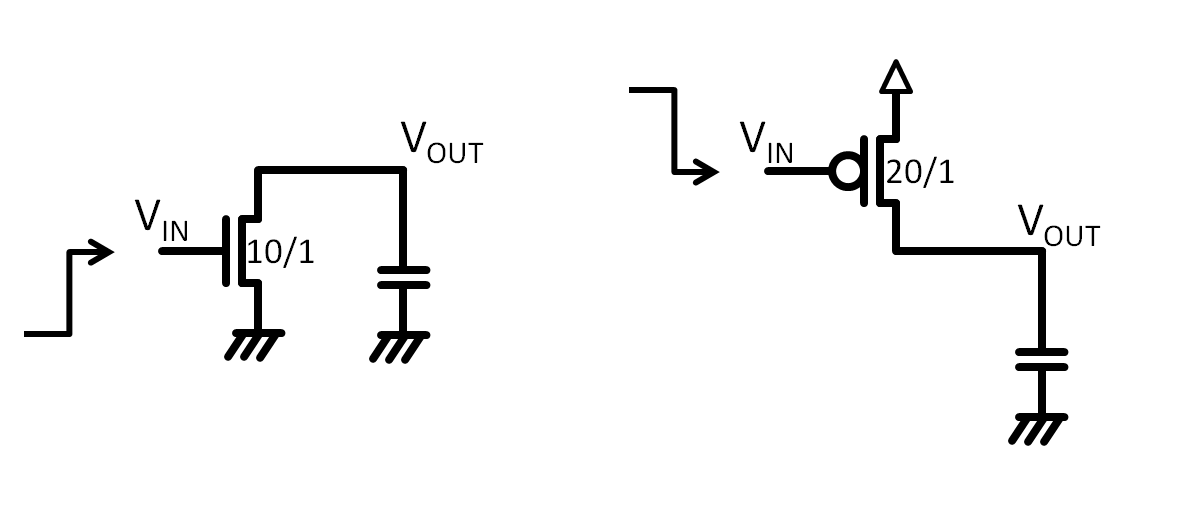
\includegraphics[width=10cm]{figures/fig7-1.png}
   	\caption{Exercice 1}
   	\label{fig7-1}
\end{figure}

Calculez les délais à 50\% des transitions symbolisées sur la figure~\ref{fig7-1}
pour des transistors à canaux court en technologie 50nm avec $C_{ox}$=62.5aF/$\mu m^2$,
$R_n$=34k$\Omega\mu$m et $R_p$=68k$\Omega\mu$m.
Les tailles des NMOS valent $W=10\mu$m et $L=1\mu$m tandis que celles des PMOS valent
$W=20\mu$m et $L=1\mu$m.

\hspace{1cm}\hrule

\paragraph{NMOS}
Si initialement $V_{IN} = \SI{0}{\volt}$, on suppose que la capacité de charge,
$C_L$, est chargée à $V_{DD}$ (sinon, pas de transition à la sortie quand $V_{IN}$
passe à $V_{DD}$). En utilisant le modèle digital simple du MOSFET avec les
capacités parasites (section 10.1 du Baker), on obtient le circuit suivant.

\begin{center}
	\begin{tikzpicture}
		\draw
    	%(0, 2) node[anchor=east] {$V_{IN}$} to [short, o-] (1, 2)
    	%(1, 2) to [C=$\frac{3}{2}C_{ox}$] (1, 0)
    	%(1, 0) -- (4, 0)
    	(4, 0) to [R=$R_n$] (4, 2)
    	(4, 2) to [switch] (6,2)
    	(6, 2) to [C=$C_{ox}$] (6,0) -- (4, 0)
    	(6, 2) -- (8, 2) to [C=$C_L$] (8,0) -- (6, 0)
    	(8, 2) to [short, -o] (9,2) node[anchor=west] {$V_{OUT}$}
    	(6, 0) node[ground] {};
	\end{tikzpicture}
\end{center}

Toujours selon ce même modèle digital simple du MOSFET, le switch se ferme
quand $V_{GS} = V_{IN} > \frac{V_{DD}}{2}$.
Soit $C_{tot} = C_L + C_{ox}$ la mise en parallèle de $C_L$ et $C_{ox}$. Le
circuit, une fois le switch fermé, se résume à un simple circuit RC.
Notons que la capacité $C_{ox}$ vient du théorème de Miller appliqué
à $C_{GD}$ où $C_{GD}$ est grossièrement approximée par $C_{ox}/2$.

\begin{center}
	\begin{tikzpicture}
		\draw
    	(0, 0) to [R=$R_n$] (0, 2)
    	(0, 0) -- (2, 0)
    	(2, 0) to [C=$C_{tot}$] (2, 2) -- (0, 2)
    	(2, 2) to [short, -o] (3,2) node[anchor=west] {$V_{OUT}$}
    	(1, 0) node[ground] {};
	\end{tikzpicture}
\end{center}

La tension $V_{OUT}$ évolue selon l'équation différentielle
\[ \fdif{V_{OUT}}{t} + \frac{V_{OUT}}{R_nC_{tot}} = 0 \]
dont la solution est une exponentielle de constante de temps $\tau = R_nC_{tot}$
\[ V_{OUT}(t) = V_{DD}\exp\left(-t/\tau\right).\]
Soit $t_{PHL}$ le délai de propagation à 50\% de $V_{DD}$ (high) à \SI{0}{\volt} (low)
\footnote{Ce délai et les autres sont définit dans la section 10.1.3 du Baker.}.
$t_{PHL}$ est donné par
\[ V_{OUT}(t_{PHL}) = V_{DD}\exp\left(-t_{PHL}/\tau\right) = \frac{V_{DD}}{2} \]
et donc
\[ t_{PHL} = \ln(2)\cdot R_n\cdot C_{tot} \approx 0.7\cdot R_n\cdot C_{tot}. \]
\`{A} l'avenir, on utilisera directement cette approximation sans repasser par le calcul
complet (mais faire une fois ce calcul permet de voir d'où elle vient).

La résistance $R'_n$ donnée dans l'énoncé doit encore être divisée par $W$ pour
obtenir $R_n$
\[ R_n = \frac{R'_n}{W}. \]
Cette formule n'est cependant valable que pour $L=1$ (notons que $L=1$ veut
dire que la longueur du transistor est de \SI{50}{\nano\meter}, comme le
scale factor est de \SI{50}{\nano\meter}). Ici, la longueur du transistor
est de $\SI{1}{\micro\meter}$, soit $L=20$, on a donc finalement
\[ R_n = \SI{34}{\kilo\ohm\micro\meter}\frac{20}{\SI{10}{\micro\meter}} =
\SI{68}{\kilo\ohm}. \]
Ensuite, pour obtenir $C_{ox}$, il faut multiplier $C'_{ox}$ par la surface du
transistor $WL$
\[ C_{ox} = C'_{ox}\cdot(WL) = \SI{625}{\atto\farad}. \]
Comme $C_L$ n'est pas donnée dans l'énoncé, on suppose $C_L = \SI{50}{\femto\farad}$.
Enfin, le délai est donné par
\[ t_{PHL} = \SI{2.41}{\nano\second}. \]

\paragraph{PMOS}
Pour le PMOS, le raisonnement est exactement identique. On suppose cette fois que la
capacité de charge $C_L$ est initialement chargée à \SI{0}{\volt}. Le modèle digital
simple du MOSFET appliqué au PMOS nous donne le circuit suivant.

\begin{center}
	\begin{tikzpicture}
		\draw
    	(0, 4) node[vcc] {$V_{DD}$} to [R=$R_p$] (0, 2)
    	(0, 2) to [switch] (3, 2)
    	(3, 2) to [C=$C_{ox}$] (3, 4) node[vcc] {$V_{DD}$}
    	(3, 2) -- (4, 2) to [C=$C_L$] (4,0) node[ground] {}
    	(4, 2) to [short, -o] (5, 2) node[anchor=west] {$V_{OUT}$};
	\end{tikzpicture}
\end{center}

Le switch se ferme cette fois dès que $V_{SG} = V_{DD} - V_{IN} > \frac{V_{DD}}{2}$.
Une fois ce switch fermé, le circuit se résume à nouveau à un simple circuit RC.

\begin{center}
	\begin{tikzpicture}
		\draw
    	(0, 4) node[vcc] {$V_{DD}$} to [R=$R_p$] (0, 2)
    	(0, 2) -- (3, 2)
    	(3, 2) to [C=$C_{ox}$] (3, 4) node[vcc] {$V_{DD}$}
    	(3, 2) -- (4, 2) to [C=$C_L$] (4,0) node[ground] {}
    	(4, 2) to [short, -o] (5, 2) node[anchor=west] {$V_{OUT}$};
	\end{tikzpicture}
\end{center}

Soit $C_{tot} = C_L + C_{ox}$. L'équation différentielle régissant la variation
de $V_{OUT}$ est donnée par
\[ \fdif{V_{OUT}}{t} + \frac{V_{OUT}}{R_pC_{tot}} = \frac{V_{DD}}{R_pC_{tot}} \]
et donc, en notant $\tau = R_nC_{tot}$,
\[ V_{OUT}(t) = V_{DD}\left(1 - \exp\left(-t/\tau\right)\right). \]
Le délai $t_{PLH}$ est donné par
\[ V_{OUT}(t_{PLH}) = V_{DD}\left(1 - \exp\left(-t_{PLH}/\tau\right)\right) = \frac{V_{DD}}{2} \]
et donc
\[ t_{PLH} = \ln(2)\cdot R_p\cdot C_{tot} \approx 0.7\cdot R_p\cdot C_{tot}. \]
De la même manière que pour le NMOS,
\[ R_p = \SI{68}{\kilo\ohm\micro\meter}\frac{20}{\SI{20}{\micro\meter}} =
\SI{68}{\kilo\ohm}. \]
Ensuite,
\[ C_{ox} = C'_{ox}\cdot(WL) = \SI{1.25}{\femto\farad}. \]
Finalement,
\[ t_{PLH} = \SI{2.44}{\nano\second}. \]

\paragraph{Remarque} On voit donc que dimensionner le PMOS en choisissant une
largeur deux fois plus grande que pour le NMOS permet d'avoir $t_{PHL} \approx
t_{PLH}$ (en négligeant les capacités parasites par rapport à la capacité
de charge, on a même $t_{PHL} = t_{PLH}$). Cependant, cela a aussi pour effet
d'augmenter la capacité d'entrée $C_{in} = \frac{3}{2}C_{ox}$ du circuit avec
le PMOS.

\newpage
\section*{Exercice 2: inverseur CMOS}

On considère une chaîne d'inverseurs CMOS identiques avec ses pistes d'interconnexion
en technologie 0.18$\mu$m, comme représenté à la figure~\ref{fig7-2}. Voici les paramètres
technologiques :

\begin{center}
$
	\begin{array}{l l l}
		L_{min} = 0.18 \mu m 	& V_{DD} = 1.8 V 		& V_{t0,n} = |V_{t0,p} | = 0.5 V \\
		\mu_n = 0.04 m^2/Vs 	& \mu_p = 0.02 m^2/Vs	& C_{ox} = 5 fF/\mu m^2 \\
		C_{rout} = 10fF			&						& \\
	\end{array}
$
\end{center}

\begin{figure}[!htbp]
   \centering
   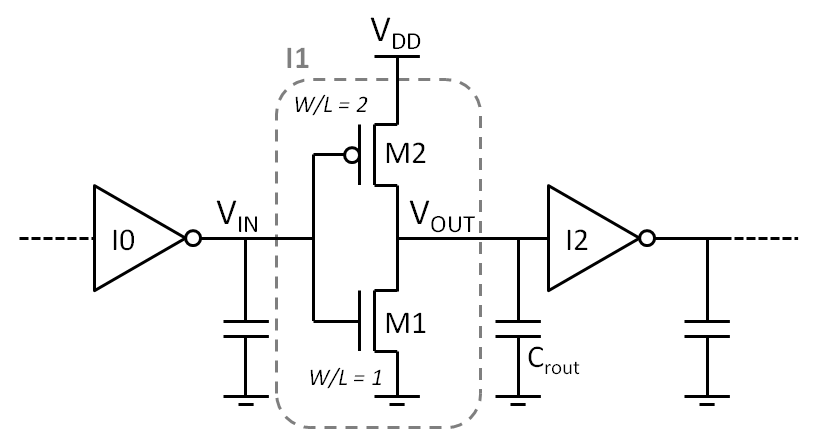
\includegraphics[width=10cm]{figures/fig7-2.png}
   \caption{Exercice 1}
   \label{fig7-2}
\end{figure}

\emph{Analyse DC}
\begin{enumerate}
	\item Pour une transition infiniment lente à l'entrée de I1, déterminez le régime de
	fonctionnement de M1 et M2 ainsi que la tension $V_{OUT}$ en fonction de $V_{IN}$.
\end{enumerate}

\emph{Délai de propagation}
\begin{enumerate}
	\setcounter{enumi}{1}
	\item Comme estimation du délai de propagation ($t_p$) de I1, on vous demande de
	calculer le temps de descente de $V_{OUT}$ à 50\% lors d'un flanc montant sur $V_{IN}$
	($t_{PHL}$) sachant que $R'_n =13.8$k$\Omega\mu$m.
	%\item Comme estimation du délai de propagation ($t_p$) de I1, on vous demande de
	%calculer le temps de descente de \vout à 50\% lors d'un flanc montant sur \vin
	%($t_{PHL}$). Pour ce faire, remplacer M1 et M2 par des éléments plus simples
	%(résistance, sources) en fonction du régime de fonctionnement. On suppose que
	%le flanc sur \vin est idéal et on néglige les capacités parasites.
	%\item On souhaite simplifier le calcul du délai de propagation en remplaçant M1
	%par une résistance équivalente $R_{eq}$ qui donne la même valeur de délai que
	%celle trouvée précédemment. Pour ce faire, on vous demande de trouver un facteur
	%de fitting k pour exprimer $R_{eq}$ en fonction de la résistance en mode linéaire
	%:\\ $R_{eq}$ = k $R_{lin}$ .
\end{enumerate}

\emph{Scaling de la technologie CMOS}
\begin{enumerate}
	\setcounter{enumi}{2}
	\item Répeter le point précédent pour les paramètres ci-dessous en sachant que
	$R'_n = 464$k$\Omega\mu$m.
	%\item On considère cette fois une technologie 65nm avec les paramètres ci-dessous.
	%Calculer le délai sur base de la formule obtenue au point c). Négliger les capacités parasites.

	\begin{center}
	$
		\begin{array}{l l l}
			L_{min} = 65 nm 		& V_{DD} = 1.2V 		&V_{t0,n} = |V_{t0,p}| = 0.4V \\
			\mu_n = 0.05 m^2/Vs 	& \mu_p= 0.025 m^2/Vs	& C_{ox} = 7 fF/\mu m^2 \\
			C_{rout} = 2fF			&						& \\
		\end{array}
	$
	\end{center}
\end{enumerate}

\hspace{1cm}\hrule

\subsection*{Question 1: Analyse DC}
\subsubsection*{Approche mathématique rigoureuse}
\paragraph{Calcul des paramètres}
\begin{align*}
    k_n &= \left(\frac{W}{L}\right)_n \mu_n C_{ox} = \SI{200}{\micro A/V^2} \\
    k_p &= \left(\frac{W}{L}\right)_p \mu_p C_{ox} = \SI{200}{\micro A/V^2} \\
\end{align*}

\og Transition infiniment lente\fg signifie que l'on analyse ce qu'il se passe
en DC, pour différentes valeurs de l'entrée (ce que fait SPICE pour une analyse
\texttt{.DC}).

On est en DC, en grand signal, le courant de sortie est donc nul (la sortie est
connectée à des capacités). Les courants dans les deux transistors sont donc
égaux.

\paragraph{Pour $V_{IN} < V_{t0,n}$:}
M1 est bloqué et M2 est passant.
Comme $I_{2} = 0$, le M2 ne peut pas être en saturation,
donc il est en triode:
\[I_{OUT} = k_p \left(V_{OV,M2} - \frac{1}{2} V_{SD,M2}\right)V_{SD,M2} = \SI{0}{A}\]
On a donc $V_{SD,M2} = \SI{0}{V}$, et donc $V_{OUT} = V_{DD}$.

\paragraph{Pour $V_{IN} > V_{DD} - \left|V_{t0,p}\right|$:}
M2 est bloqué et M1 passant. Par un raisonnement similaire à ci-dessus,
on trouve $V_{OUT} = \SI{0}{V}$.

\paragraph{Pour $V_{t_0,n} < V_{IN} < V_{DD} - \left|V_{t0,p}\right|$:}
Les deux transistors sont passants.

En partant de $V_{IN} = V_{DD} - \left|V_{t0,p}\right|$,
si on diminue $V_{IN}$, M1 reste en triode et M2 devient passant
(en saturation car $V_{SD} \approx V_{DD}$, alors que $V_{OV} \approx \SI{0}{V}$).

On a donc
\begin{align*}
    I_{M1} &= k_n \left(V_{OV,M1}-\frac{1}{2}V_{DS,M1}\right)V_{DS,M1} \\
    I_{M2} &= \frac{k_p}{2} V_{OV,M2}^2 \\
    I_{M1} &= I_{M2} \\
\end{align*}

On peut donc résoudre ce système pour trouver $V_{OUT}$ en fonction
de $V_{IN}$ (en utilisant $k_n = k_p$ et $V_t = V_{t0,n} = |V_{t0,p}|$:
\[V_{OUT} = V_{IN}-V_t - \sqrt{(V_{IN}-V_t)^2-(V_{DD}-V_{IN}-V_t)^2}.\]

La limite de ce régime de fonctionnement est atteinte quand
$V_{OV,M2} = V_{SD,M2}$, donc $\frac{k_p}{2}V_{OV,M2}^2 = \frac{k_n}{2}V_{OV,M1}^2$.
Comme $k_n = k_p$, cela donne $V_{IN} = V_{DD}/2$.

Si on diminue encore $V_{IN}$, on rentre dans une zone où les deux transistors sont en saturation.
Sans connaitre les paramètres de l'effet Early, on ne peut pas calculer
$V_{OUT}$ en fonction de $V_{IN}$ (si on néglige l'effet Early, on
obtient une caractéristique $V_{OUT}(V_{IN})$ verticale pour cette région,
ce qui n'a pas pas de sens physique).

Quand $V_{IN}$ est suffisament petit, on arrive dans une région où
M1 est en saturation et M2 en triode.
Les équations sont alors
\begin{align*}
    I_{M1} &= \frac{k_n}{2} (V_{IN} - V_{t0,n})^2 \\
    I_{M2} &= k_p \left(V_{OV,M2}-\frac{1}{2}V_{SD,M2}\right)V_{SD,M2} \\
    I_{M1} &= I_{M2} \\
\end{align*}

On peut alors tracer la courbe DC de l'inverseur CMOS (voir figure~\ref{fig:dc-inv}).
\begin{figure}
	\centering
	\includegraphics[width=0.7\textwidth,height=0.5\textwidth]{figures/ex2_1.tikz}
	\caption{Caractéristique entrée-sortie de l'inverseur CMOS.}
	\label{fig:dc-inv}
\end{figure}

\subsubsection*{Approche via diagramme de Jespers}
Un diagramme de Jespers permet d'obtenir de façon visuelle les différents régimes
de fonctionnement d'un ou plusieurs transistors en fonction des tensions $V_G$
(qu'on indique sur l'axe des $y$) et $V_D$ et $V_S$ (qu'on indique sur l'axe des $x$).
Même sans faire aucun calcul, on sait que la caractéristique entrée sortie de l'inverseur
CMOS aura une allure similaire à celle présente sur la figure~\ref{fig:dc-inv}. Grâce à
cela et au fait que $I_{M1} = I_{M2}$, on va pouvoir utilser un diagramme de Jespers
pour trouver les régimes de fonctionnement de M1 et M2 selon $V_{IN}$. Avant tout, on note
que $V_{IN} = V_{G1} = V_{G2} = V_G$ et $V_{OUT} = V_{D1} = V_{D2} = V_D$.

Dans le diagramme de Jespers, le courant traversant M1 est donnée par l'aire de la
surface comprise entre les droites $y = V_G$, $x = V_{S1}$, $x = V_D$ au dessus de 
$y=V_{t0,n}+x$ (au facteur $k_n$ près) tandis que le courant traversant M2 est donnée par
l'aire de la surface comprise entre les droites $y = V_G$, $x = V_{S2}$, $x = V_D$ en
dessous de $y=-|V_{t0,p}|+x$ (au facteur $k_p$ près). Si cette surface est un triangle, on est
en saturation. Si cette surface est un trapèze, on est en triode. Dans tous les cas,
comme $I_{M1} = I_{M2}$ \emph{et} que $k_n = k_p$, ces deux surfaces doivent être égales.

Dans le cas où $V_{IN} < V_{t0,n}$ (figure~\ref{fig:jsp1}), M1 est clairement bloqué (pas de
surface au dessus de $y=V_{t0,n}+x$). On a aussi (via la caractéristique entrée-sortie)
$V_{OUT} = V_{DD}$. La surface comprise entre $y = V_G$, $x = V_{S2}$, $x = V_D$
en dessous de $y=-|V_{t0,p}|+x$  est dans ce cas un trapèze de hauteur nulle.
On peut donc déjà dire que pour $V_{IN} \in [0, V_{t0,n}[$, M1 est coupé alors que
M2 est en triode.

\begin{figure}[ht]
	\centering
	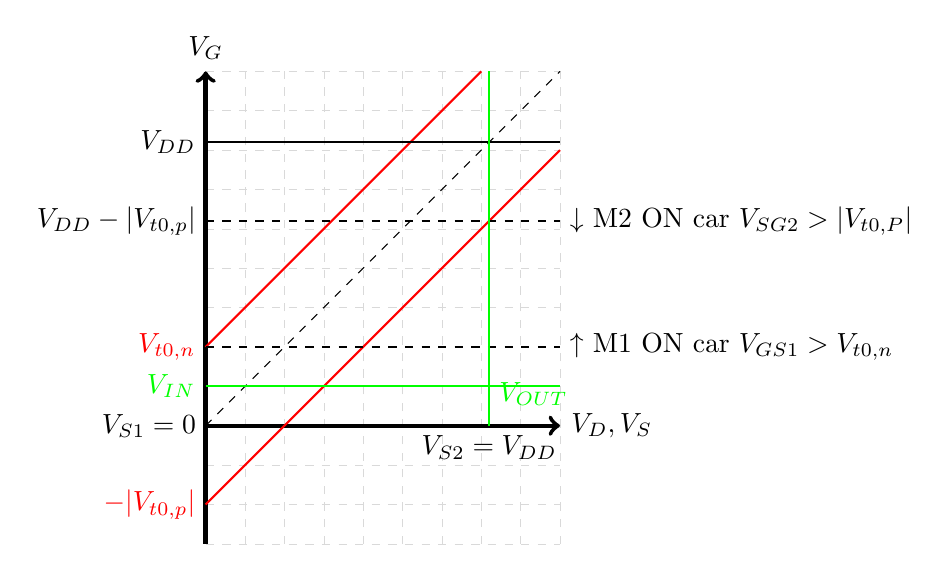
\begin{tikzpicture}[scale=0.5]
		%% Compared to the statements, everything is multiplied by 4
		\draw[help lines, color=gray!30, dashed] (0,-3) grid (9,9);
		\draw[->,ultra thick] (0,0)--(9,0) node[right]{$V_D, V_S$};
		\draw[->,ultra thick] (0,-3)--(0,9) node[above]{$V_G$};
		
		%% Threshold voltages
		\draw[dashed] (0,0) node[left]{$V_{S1} = 0$} --(9,9);
		\draw[thick,red] (0,2) node[left]{$V_{t0,n}$} --(7,9);
		\draw[thick,red] (0,-2) node[left]{$-|V_{t0,p}|$} --(9,7);

		%% VDD
		\draw[thick] (7.2,0) node[below]{$V_{S2} = V_{DD}$} --(7.2,9);
		\draw[thick] (0,7.2) node[left]{$V_{DD}$} -- (9,7.2);
		
		% Off limits for M1 and M2
		\draw[dashed] (0,2) -- (9,2) node[right]
		{$\uparrow$ M1 ON car $V_{GS1} > V_{t0,n}$};
		\draw[dashed] (0,5.2) node[left]{$V_{DD}-|V_{t0,p}|$} -- (9,5.2) node[right]
		{$\downarrow$ M2 ON car $V_{SG2} > |V_{t0,P}|$};
		
		% VIN, VOUT
		\draw[thick, green] (0,1) node[left] {$V_{IN}$} -- (9,1);
		\draw[thick, green] (7.2,0) node[above, right, yshift=0.4cm] {$V_{OUT}$} -- (7.2,9);
	\end{tikzpicture}
	\caption{Diagramme de Jespers pour $V_{IN} < V_{t0,n}$. M1 est off tandis que M2
	est en triode (la surface représentant le courant est un trapèze de hauteur nulle).}
	\label{fig:jsp1}
\end{figure}

Si $V_{IN}$ devient maintenant $> V_{t0,n}$ (figure~\ref{fig:jps2}), M1 devient passant et en saturation
tandis que M2 reste en triode. Ce sera le cas jusqu'à ce que M2 passe aussi en
saturation. M2 passera en saturation quand la tension $V_{OUT}$ sera assez éloignée de $V_{DD}$
pour que la surface représentant le courant traversant M2 soit un triangle. Cela se produit
pour $V_{IN} = V_{DD}/2$. Donc, pour $V_{IN} \in [V_{t0,n}; V_{DD}/2[$,
M1 est en saturation tandis que M2 est en triode.

\begin{figure}[ht]
	\centering
	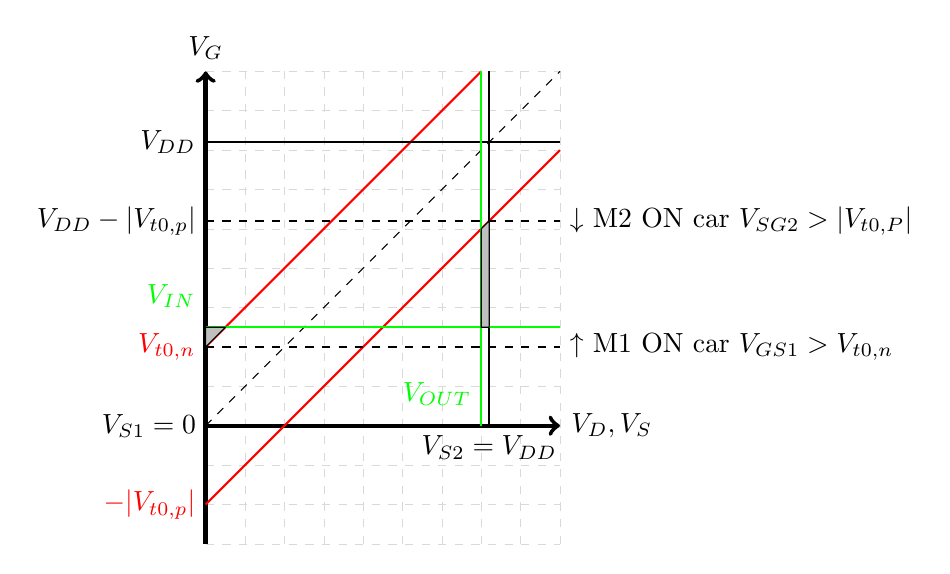
\begin{tikzpicture}[scale=0.5]
		%% Compared to the statements, everything is multiplied by 4
		\draw[help lines, color=gray!30, dashed] (0,-3) grid (9,9);
		\draw[->,ultra thick] (0,0)--(9,0) node[right]{$V_D, V_S$};
		\draw[->,ultra thick] (0,-3)--(0,9) node[above]{$V_G$};
		
		%% Threshold voltages
		\draw[thick,red] (0,2) node[left]{$V_{t0,n}$} --(7,9);
		\draw[thick,red] (0,-2) node[left]{$-|V_{t0,p}|$} --(9,7);

		%% VDD
		\draw[dashed] (0,0) node[left]{$V_{S1} = 0$} --(9,9);
		\draw[thick] (7.2,0) node[below]{$V_{S2} = V_{DD}$} --(7.2,9);
		\draw[thick] (0,7.2) node[left]{$V_{DD}$} -- (9,7.2);
		
		% Off limits for M1 and M2
		\draw[dashed] (0,2) -- (9,2) node[right]
		{$\uparrow$ M1 ON car $V_{GS1} > V_{t0,n}$};
		\draw[dashed] (0,5.2) node[left]{$V_{DD}-|V_{t0,p}|$} -- (9,5.2) node[right]
		{$\downarrow$ M2 ON car $V_{SG2} > |V_{t0,P}|$};
		
		% VIN, VOUT
		\draw[thick, green] (0,2.5) node[left, yshift=0.4cm] {$V_{IN}$} -- (9,2.5);
		\draw[thick, green] (7,0) node[above, left, yshift=0.4cm] {$V_{OUT}$} -- (7,9);
		
		\draw[fill=gray!50] (0,2) -- (0,2.5) -- (0.5,2.5) -- cycle;
		\draw[fill=gray!50] (7,2.5) -- (7,5) -- (7.2, 5.2) -- (7.2,2.5) -- cycle;
	\end{tikzpicture}
	\caption{Diagramme de Jespers pour $V_{IN} \in [V_{t0,n}, V_{DD/2}[$. M1 est en
	saturation tandis que M2 est en triode. Note: les surfaces grises ont, en théorie,
	une surface égale. Ce n'est pas forcément le cas sur cette figure par imprécision.}
	\label{fig:jps2}
\end{figure}

Le diagramme de Jespers pour $V_{IN} = V_{DD}/2$ est repris à la figure~\ref{fig:jsp3}, on
voit bien que les deux transistors sont ici en saturation.

\begin{figure}[ht]
	\centering
	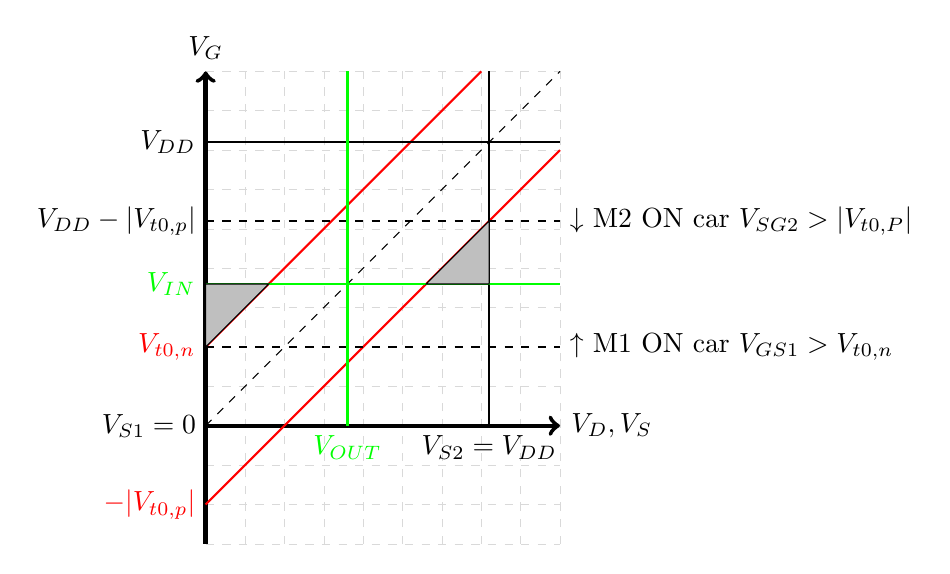
\begin{tikzpicture}[scale=0.5]
		%% Compared to the statements, everything is multiplied by 4
		\draw[help lines, color=gray!30, dashed] (0,-3) grid (9,9);
		\draw[->,ultra thick] (0,0)--(9,0) node[right]{$V_D, V_S$};
		\draw[->,ultra thick] (0,-3)--(0,9) node[above]{$V_G$};
		
		%% Threshold voltages
		\draw[thick,red] (0,2) node[left]{$V_{t0,n}$} --(7,9);
		\draw[thick,red] (0,-2) node[left]{$-|V_{t0,p}|$} --(9,7);

		%% VDD
		\draw[dashed] (0,0) node[left]{$V_{S1} = 0$} --(9,9);
		\draw[thick] (7.2,0) node[below]{$V_{S2} = V_{DD}$} --(7.2,9);
		\draw[thick] (0,7.2) node[left]{$V_{DD}$} -- (9,7.2);
		
		% Off limits for M1 and M2
		\draw[dashed] (0,2) -- (9,2) node[right]
		{$\uparrow$ M1 ON car $V_{GS1} > V_{t0,n}$};
		\draw[dashed] (0,5.2) node[left]{$V_{DD}-|V_{t0,p}|$} -- (9,5.2) node[right]
		{$\downarrow$ M2 ON car $V_{SG2} > |V_{t0,P}|$};
		
		% VIN, VOUT
		\draw[thick, green] (0,3.6) node[left] {$V_{IN}$} -- (9,3.6);
		\draw[thick, green] (3.6,0) node[below] {$V_{OUT}$} -- (3.6,9);
		
		\draw[fill=gray!50] (0,2) -- (0,3.6) -- (1.6,3.6) -- cycle;
		\draw[fill=gray!50] (5.6,3.6) -- (7.2,5.2) -- (7.2, 3.6) -- cycle;
	\end{tikzpicture}
	\caption{Diagramme de Jespers pour $V_{IN} = V_{DD}/2$. M1 et M2 sont en saturation.
	On voit que c'est le cas pour toute une gamme de valeurs de $V_{OUT}$, cela correspond
	bien à la pente infinie en $V_{IN} = V_{DD}/2$ obtenue sur la caractéristique entrée-sortie
	de la figure~\ref{fig:dc-inv}.}
	\label{fig:jsp3}
\end{figure}

Pour $V_{IN} > V_{DD}/2$ (figure~\ref{fig:jsp4}), M1 passe en régime triode tandis
que M2 reste en saturation.

\begin{figure}[ht]
	\centering
	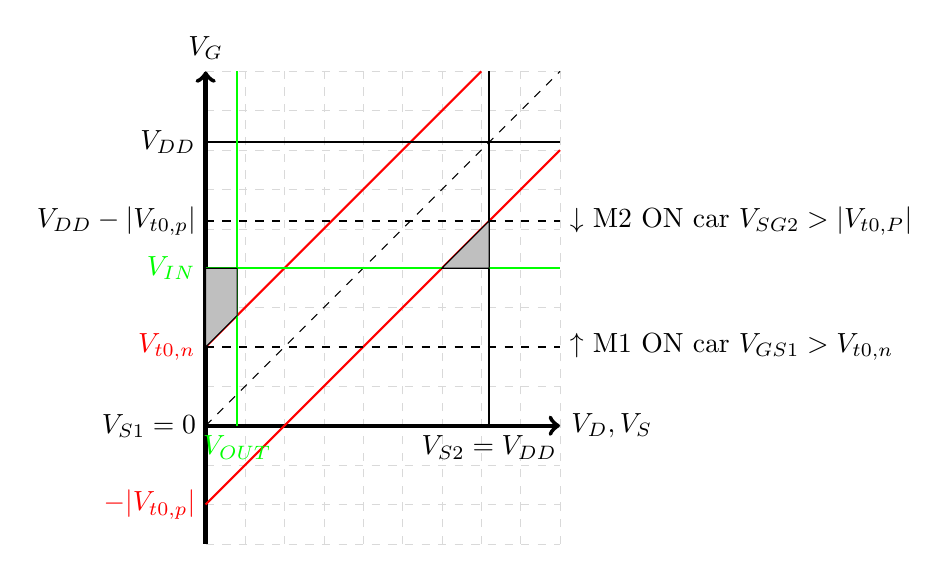
\begin{tikzpicture}[scale=0.5]
		%% Compared to the statements, everything is multiplied by 4
		\draw[help lines, color=gray!30, dashed] (0,-3) grid (9,9);
		\draw[->,ultra thick] (0,0)--(9,0) node[right]{$V_D, V_S$};
		\draw[->,ultra thick] (0,-3)--(0,9) node[above]{$V_G$};
		
		%% Threshold voltages
		\draw[thick,red] (0,2) node[left]{$V_{t0,n}$} --(7,9);
		\draw[thick,red] (0,-2) node[left]{$-|V_{t0,p}|$} --(9,7);

		%% VDD
		\draw[dashed] (0,0) node[left]{$V_{S1} = 0$} --(9,9);
		\draw[thick] (7.2,0) node[below]{$V_{S2} = V_{DD}$} --(7.2,9);
		\draw[thick] (0,7.2) node[left]{$V_{DD}$} -- (9,7.2);
		
		% Off limits for M1 and M2
		\draw[dashed] (0,2) -- (9,2) node[right]
		{$\uparrow$ M1 ON car $V_{GS1} > V_{t0,n}$};
		\draw[dashed] (0,5.2) node[left]{$V_{DD}-|V_{t0,p}|$} -- (9,5.2) node[right]
		{$\downarrow$ M2 ON car $V_{SG2} > |V_{t0,P}|$};
		
		% VIN, VOUT
		\draw[thick, green] (0,4) node[left] {$V_{IN}$} -- (9,4);
		\draw[thick, green] (0.8,0) node[below] {$V_{OUT}$} -- (0.8,9);
		
		\draw[fill=gray!50] (0,2) -- (0,4) -- (0.8,4) -- (0.8,2.8) -- cycle;
		\draw[fill=gray!50] (6,4) -- (7.2,5.2) -- (7.2, 4) -- cycle;
	\end{tikzpicture}
	\caption{Diagramme de Jespers pour $V_{IN} \in ]V_{DD}/2, V_{DD}-|V_{t0,p}|[$.
	M1 est en triode, M2 en saturation.}
	\label{fig:jsp4}
\end{figure}

Enfin, pour $V_{IN} > V_{DD}-|V_{t0,n}|$ (figure ~\ref{fig:jsp5}), M1 est en triode
mais est traversé par un courant nul (trapèze de hauteur nulle dans le diagramme de
Jespers) tandis que M2 est off.

\begin{figure}[ht]
	\centering
	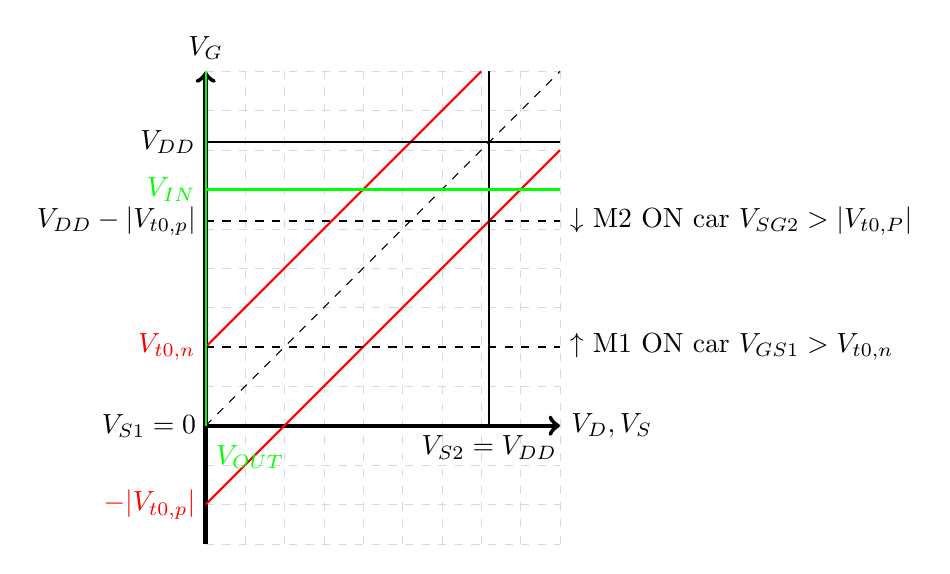
\begin{tikzpicture}[scale=0.5]
		%% Compared to the statements, everything is multiplied by 4
		\draw[help lines, color=gray!30, dashed] (0,-3) grid (9,9);
		\draw[->,ultra thick] (0,0)--(9,0) node[right]{$V_D, V_S$};
		\draw[->,ultra thick] (0,-3)--(0,9) node[above]{$V_G$};
		
		%% Threshold voltages
		\draw[thick,red] (0,2) node[left]{$V_{t0,n}$} --(7,9);
		\draw[thick,red] (0,-2) node[left]{$-|V_{t0,p}|$} --(9,7);

		%% VDD
		\draw[dashed] (0,0) node[left]{$V_{S1} = 0$} --(9,9);
		\draw[thick] (7.2,0) node[below]{$V_{S2} = V_{DD}$} --(7.2,9);
		\draw[thick] (0,7.2) node[left]{$V_{DD}$} -- (9,7.2);
		
		% Off limits for M1 and M2
		\draw[dashed] (0,2) -- (9,2) node[right]
		{$\uparrow$ M1 ON car $V_{GS1} > V_{t0,n}$};
		\draw[dashed] (0,5.2) node[left]{$V_{DD}-|V_{t0,p}|$} -- (9,5.2) node[right]
		{$\downarrow$ M2 ON car $V_{SG2} > |V_{t0,P}|$};
		
		% VIN, VOUT
		\draw[thick, green] (0,6) node[left] {$V_{IN}$} -- (9,6);
		\draw[thick, green] (0,0) node[below, right, yshift=-0.4cm] {$V_{OUT}$} -- (0,9);
	\end{tikzpicture}
	\caption{Diagramme de Jespers pour $V_{IN} \in [V_{DD}-|V_{t0,p}|, V_{DD}]$.
	M1 est en triode mais est traversé par un courant nulle (trapèze de hauteur nulle),
	M2 en off.}
	\label{fig:jsp5}
\end{figure}

\subsection*{Question 2: Délai de propagation}
$t_{PHL} \approx 0.7R_nC_{tot} = $

\subsection*{Question 3: Scaling de la technologie CMOS}
$t_{PHL} \approx 0.7R_nC_{tot} = $

\newpage
\section*{Exercice 3 : logique de passage}
On considère les 3 implémentations d'un multiplexeur 2 vers 1 de la figure~\ref{fig7-3} :
transmission gate, pass gate et static CMOS gate. La fonction logique associée est :
Y = (Sel.A) + ($\overline{Sel}$.B) et la technologie considérée est une technologie
0.18 $\mu$m avec les paramètres suivants:

\begin{center}
$
	\begin{array}{l l l}
		L_{min} = 0.18 \mu m 	& V_{DD} = 1.8 V 		& V_{t0,n} = |V_{t0,p} | = 0.5 V \\
		\mu_n = 0.04 m^2/Vs 	& \mu_p = 0.02 m^2/Vs	& C_{ox} = 5 fF/\mu m^2 \\
		C_{rout} = 10fF			&						& \\
	\end{array}
$
\end{center}

\begin{figure}[!htbp]
   \centering
   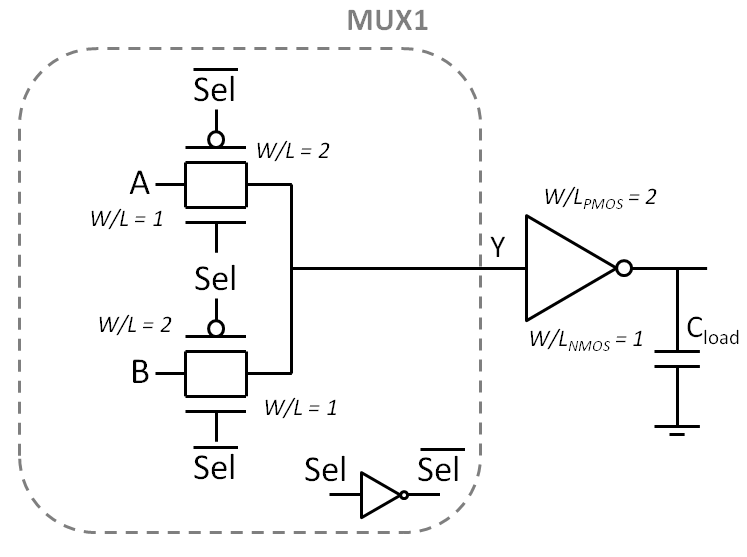
\includegraphics[width=9cm]{figures/fig7-3-1.png}
	 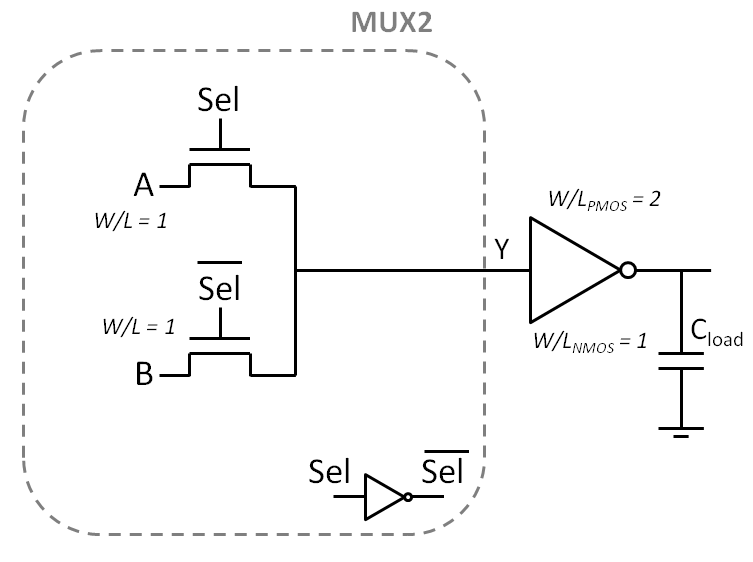
\includegraphics[width=9cm]{figures/fig7-3-2.png}
	 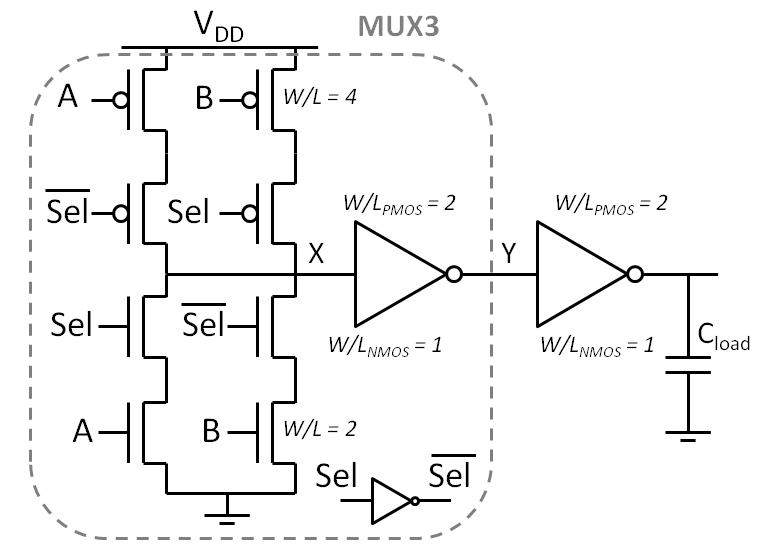
\includegraphics[width=9cm]{figures/fig7-3-3.png}
   \caption{Exercice 1}
   \label{fig7-3}
\end{figure}

\begin{enumerate}
	\item Déterminer les tensions des niveaux logiques haut ($V_{OH}$) et bas ($V_{OL}$) de
	la sortie Y pour chacun de ces multiplexeurs.
	\item Calculez le temps de décharge à 50\% ($t_{PHL}$) de la capacité $C_{load}$ par
	l'inverseur de l'étage suivant, suite à un flanc montant à la sortie Y. Considérez une
	résistance équivalente pour les transistors passant du régime saturé au linéaire de
	$R_{eq}$ = 2.5 $R_{lin}$ et négliger toutes les capacités parasites.
\end{enumerate}

\hspace{1cm}\hrule

\subsection*{Niveaux logiques}
\paragraph{MUX1: transmission gate} 
Ce multiplexeur est composé de deux transmission gates (TG).
Une TG combine un transistor NMOS et un transistor PMOS de façon à se débarasser
de leurs défauts lorsque ces transistors sont utilisés individuellement dans une
simple pass gate (PG). En effet, on sait qu'un NMOS passe bien un "0" mais ne passe
pas bien un "1". Au contraire, un PMOS passe bien un "1" mais ne passe pas bien un "0".
Dans une TG, les "1" et "0" passent tous les deux bien grâce à l'association PMOS/NMOS.
On a donc
\begin{align*}
	V_{OL} &= \SI{0}{\volt} & V_{OH} &= V_{DD}.
\end{align*}

\paragraph{MUX2: pass gate} 
\`{A} l'inverse du MUX1, MUX2 utilise de simple pass gates NMOS.
Comme expliqué précédemment, un NMOS ne passe pas bien un "1". Ici, on a donc
\begin{align*}
	V_{OL} &= \SI{0}{\volt} & V_{OH} &= V_{DD}-V_{t0,n}.
\end{align*}

\paragraph{MUX3: static CMOS gate}
Ici, on constate que les NMOS ne font passer que des "0" et que les PMOS ne
font passer que des "1". On se retrouve donc à nouveau avec
\begin{align*}
	V_{OL} &= \SI{0}{\volt} & V_{OH} &= V_{DD}.
\end{align*}

\subsection*{Temps de décharge}
Voir l'exercice 2.4.
\[R_{eq} = k R_{lin} = \frac{k}{k_n (V_{DD} - V_t)} = \SI{9.62}{\kilo\ohm} \]
\[t_{PHL} = \SI{66.6}{\pico\second} \]

\end{document}

